\documentclass[10pt,twocolumn]{article}
% Every number is traceable to a file in results/manifests/ (named in the text or
% a caption). Build: tectonic main.tex  (or pdflatex + bibtex).

\usepackage[margin=0.75in]{geometry}
\usepackage{booktabs}
\usepackage{amsmath}
\usepackage{graphicx}
\usepackage[hidelinks]{hyperref}

\title{Inspecting Parts from Ten Good Photographs on a Laptop CPU:\\
Frozen CLIP Features, an Append-Only Memory, and What It Costs}
\author{Mounika Reddy \and Ashi Sharma\\[2pt]
\normalsize [Department], [Institution]}
\date{}

\begin{document}
\maketitle

\begin{abstract}
We ask whether a small manufacturer can start automated visual inspection with
nothing more than a few photographs of good parts and the laptop it already has.
Our detector keeps a frozen OpenCLIP image encoder, stores the patch features of
1--10 normal photos in a separate memory for each product, and flags test patches
that resemble none of them; it trains nothing. We evaluate it on MVTec AD, VisA,
NEU-DET and MPDD with three backbones, FP32 and INT8, three random draws of the
support photos, and paired statistics, and we time every configuration on one
consumer CPU. With ten photos and the last transformer block, ViT-B/16 reaches
0.904 image AUROC on MVTec AD. Taking patch tokens from blocks 6, 9 and 12 as well
raises this to 0.938, and to 0.945 with windowed scoring, for under 10\% more
CPU time; the gain is similar on VisA and absent on NEU-DET and MPDD. With these
features our detection is better than that of PatchCore given the same photos on
MVTec AD, VisA and MPDD, and localisation is level on MVTec AD. On WinCLIP's
protocol we finish 2--4 points below its published few-shot results while running
the encoder once per image. Two practical findings stand out. First, the cheapest
backbone is enough exactly when defects cover more of the image than one of its
patches, which held on the three datasets where we compared backbones. Second, the laptop slows five- to
six-fold after a few minutes of continuous use, so burst latency overstates
throughput. Adding a product left every other product's scores bit-identical in
all our checks, and inspecting 10,000 parts a day costs tens of rupees of
electricity a year.
\end{abstract}

\section{Introduction}

Visual inspection in a small workshop usually means a person looking at each
part. Automating it runs into three practical problems before accuracy even
matters. When a line is new there are many good parts and almost no examples of
failures, so a method that learns from defects has nothing to learn from. The
only computer is often an office laptop, and nobody on site trains neural
networks. And the product mix changes: when a new part is introduced, inspection
of the existing parts must not be disturbed.

Anomaly detection trained on normal images addresses the first problem, and on
the MVTec AD benchmark~\cite{bergmann2019mvtec} memory-based methods such as
PatchCore~\cite{roth2022patchcore} are close to perfect. They are normally fitted
on hundreds of images per product, though, and their reported results are
accuracies. Vision--language models reduced the number of images to a
handful~\cite{jeong2023winclip}, but they were evaluated on GPUs. We could not
find a study that says how such a system behaves on a laptop CPU, what it costs
to run, or what happens to the products already being inspected when a new one is
added.

This paper is that study. We use a deliberately plain detector: a frozen CLIP
encoder~\cite{radford2021clip,cherti2023openclip} and a nearest-neighbour memory
of good patches, with two optional refinements, scoring over small windows of
patches and fusing a text prompt into the image score. We measure four things:
\begin{enumerate}
\item accuracy as a function of the number of good photos (1, 5, 10), on four
  datasets that differ in defect size and domain;
\item which backbone and precision a workshop should choose, and why;
\item the CPU cost, both for a cool machine and under continuous use;
\item whether adding a product leaves the others untouched.
\end{enumerate}
We compare against PatchCore given the same photos and against WinCLIP on its
own protocol, and we release the code, the split files and a command for every
table.

\section{Related work}

\paragraph{Learning from normal images.} MVTec AD~\cite{bergmann2019mvtec} and
VisA~\cite{zou2022visa} established the protocol of fitting on defect-free images
and testing on both kinds. PaDiM~\cite{defard2021padim} models each patch position
with a Gaussian over pretrained CNN features; PatchCore~\cite{roth2022patchcore}
stores a coreset of patch features and scores a test patch by its distance to the
nearest stored one. Our memory uses the same nearest-neighbour rule but keeps
every support patch, because a ten-photo memory is already small, and it keeps a
separate memory per product. We use anomalib's~\cite{akcay2022anomalib}
implementation of PatchCore as our baseline.

\paragraph{Vision--language models.} CLIP~\cite{radford2021clip} embeds images
and text in one space, so an image can be scored against prompts such as ``a photo
of a damaged bottle'' without any examples. WinCLIP~\cite{jeong2023winclip} adds
features computed on image windows and, with a few normal images, a reference
memory (WinCLIP+). AnomalyCLIP~\cite{zhou2024anomalyclip} instead learns prompts
that do not depend on the object. Both papers report GPU results only. We take two
ideas from WinCLIP, windows and fusing text with the memory, but compute the
windows from one encoder pass. APRIL-GAN~\cite{chen2023aprilgan} combines patch
tokens from several depths of the encoder and trains linear layers on top of
them; we take tokens from several depths as well but train nothing.

\paragraph{Adapting CLIP without training.} Tip-Adapter~\cite{zhang2022tipadapter}
turns the support features into a key--value cache for few-shot classification.
We tried its kernel as an anomaly head. At its best setting it gave exactly the
nearest-neighbour ranking, which follows from the kernel being monotonic in
cosine similarity while AUROC depends only on ranks, so we do not use it.

\section{Method}

\paragraph{Patch features.} Each image is resized to $224\times224$ and passed
through a frozen OpenCLIP ViT with OpenAI weights. The transformer's patch tokens
(768 dimensions for B/32 and B/16, 1024 for L/14) are used as they are, before
CLIP's projection to 512 dimensions; on MVTec AD the unprojected tokens scored
0.020--0.026 higher image AUROC (3.7--4.4 times the paired standard error).
B/32 gives a $7\times7$ grid of patches, B/16 $14\times14$ and L/14 $16\times16$.

\paragraph{Multi-layer features.} The last block of a CLIP ViT is trained to
summarise the whole image, which blurs where things are. Earlier blocks keep more
local detail. For ViT-B/16 we therefore also take the tokens of blocks 6 and 9,
apply the final layer norm to each block's tokens, normalise them, and concatenate
the three. The cosine between two such vectors is the mean of the three per-block
cosines. We fixed the blocks before running the experiment: half, three-quarter
and full depth, three of the four depths APRIL-GAN takes from ViT-L/14. A memory
then needs 2,304 numbers per patch instead of 768, about 18\,MB per product with
ten photos.

\paragraph{Memory and scores.} Adding a product stores the normalised patch
vectors of its $k$ good photos in a memory used only by that product. A test
patch $q$ scores
\begin{equation}
s(q) = 1 - \max_{m} \cos(q, m),
\end{equation}
the maximum running over the product's stored patches. The image score is the
largest patch score; the patch scores, bilinearly upsampled and smoothed with a
Gaussian ($\sigma = 4$), form the anomaly map. Since products share no state,
adding one cannot change another's scores, and Section~\ref{sec:incremental}
checks this directly.

\paragraph{Windows and text.} Optionally the patch vectors are average-pooled over
$2\times2$ and $3\times3$ windows and each window is scored against equally pooled
support windows; the three maps are spread back to patch resolution and averaged.
Optionally the image score becomes $0.5\,s_\text{memory} + 0.5\,s_\text{text}$,
where $s_\text{text}$ is the softmax weight that CLIP's pooled image embedding
gives to a prompt ensemble for a defective object (plus a description typed by the
user) against one for a normal object. The weight 0.5 follows WinCLIP+; we report
the full range from 0 to 1.

\paragraph{Threshold and deployment.} The application suggests a threshold by
scoring each good photo against the others and taking the largest score. The
encoder can be exported to ONNX (identical outputs to PyTorch on 50 real test
images) and quantised dynamically to INT8, which needs no calibration images.

\section{Experimental setup}

\paragraph{Data.} MVTec AD (15 products, pixel masks), VisA (12 products, pixel
masks) and NEU-DET~\cite{song2013neu} (6 classes of steel-surface defect). NEU-DET
has no defect-free class, so each class in turn is treated as normal: its support
photos come from that class, and its test set is its 60 held-out images plus 60
taken evenly from the other five classes. NEU-DET has boxes but no masks, so we
report image AUROC only. MPDD~\cite{jezek2021mpdd} has six metal parts (brackets,
connectors, plates, tubes) photographed in varied positions, orientations and
light, with pixel masks; it is the closest public benchmark to a shop floor that
we found, and we use it with B/16 only.

\paragraph{Splits and statistics.} For each product we draw 1, 5 and 10 support
photos, nested so that the smaller sets are contained in the larger ones, and keep
the whole test set fixed. This is repeated for three seeds (42, 1, 2). The split
files are in the repository. Two configurations are compared on identical
(product, shots, seed) splits; we report the mean difference and how many paired
standard errors (SE) it is, and treat a difference as real only above $2\times$SE.
For the comparison with WinCLIP we also follow its protocol on MVTec AD: 1, 2 and
4 photos and five seeds (0--4), with split files of their own.

\paragraph{Baseline.} PatchCore from anomalib (WideResNet-50-2, layers 2 and 3,
nine neighbours for re-weighting) receives exactly our support photos, test
images, masks and metric code. We switch its coreset subsampling off, since a
ten-photo memory is small and subsampling would only remove information.

\paragraph{Hardware.} All timings come from one laptop with an Intel i7-13700H
(6 performance and 8 efficiency cores), CPU only, batch size one, 6 threads, five
warm-up passes and the median of 20. With 14 threads the same graph measured 36\,ms
and 526\,ms in consecutive runs, because work landed on both core types; with six
threads repeated runs agreed within 20\%.

\section{Results}

\begin{table}[t]
\centering\small
\caption{Image / pixel AUROC with the single-pass memory, mean over three seeds
(NEU-DET: image only). Records: \texttt{benchmark} runs, paired tests in
\texttt{*\_backbones.json} and \texttt{*\_l14\_vs\_b16.json}.}
\label{tab:main}
\setlength{\tabcolsep}{4pt}
\begin{tabular}{llccc}
\toprule
 & backbone & 1 photo & 5 photos & 10 photos \\
\midrule
MVTec & B/32 & .837/.920 & .884/.934 & .904/.940 \\
      & B/16 & .856/.916 & .888/.932 & .904/.936 \\
      & L/14 & .883/.930 & .920/.942 & .933/.945 \\
\midrule
VisA  & B/32 & .681/.905 & .761/.930 & .779/.935 \\
      & B/16 & .773/.934 & .811/.947 & .831/.951 \\
      & L/14 & .785/.950 & .828/.961 & .843/.964 \\
\midrule
NEU-DET & B/32 & .818 & .867 & .893 \\
      & B/16 & .821 & .868 & .887 \\
      & L/14 & .838 & .883 & .897 \\
\bottomrule
\end{tabular}
\end{table}

\paragraph{The backbone should match the defect size.} Table~\ref{tab:main} shows
the single-pass results. On MVTec AD and NEU-DET the cheap B/32 is as accurate as
B/16: no difference reaches $2\times$SE (at ten photos, $+0.000$ on MVTec and
$-0.007$ on NEU-DET). On VisA B/16 is better at every shot count, by 0.093, 0.050
and 0.052 (4.4--5.5$\times$SE). The masks explain why. A VisA defect covers
0.04--0.9\% of the image, an MVTec AD defect 4.6\% on average, and a NEU-DET
defect box 39\%. A B/32 patch covers 2.0\% of the image and a B/16 patch 0.5\%.
When a defect is smaller than a patch, its signal is diluted by the normal pixels
around it. B/16's largest VisA gains are on its smallest-defect products. The
practical rule is simple: estimate the smallest defect that matters, and pick the
cheapest backbone whose patch is smaller than that. L/14 ($0.4\%$ per patch) is
best on MVTec AD ($+0.030$ over B/16, 4.6$\times$SE), mainly on fine defects
(\texttt{toothbrush} $+0.117$, \texttt{screw} $+0.086$), but its gains on VisA and
NEU-DET are not established, and it is 4.5 times slower.

\paragraph{More photos mainly reduce the luck of the draw.} On MVTec AD with B/16,
the standard deviation of image AUROC across seeds falls from 0.027 with one photo
to 0.012 with ten, while the mean rises by 0.048. Results from a single draw of
support photos, which many few-shot papers report, hide this spread.

\begin{table}[t]
\centering\small
\caption{What each scoring choice adds, ViT-B/16, image AUROC. Windows
$\{1,2,3\}$; text weight 0.5; ML = patch tokens from blocks 6, 9 and 12.
Records: \texttt{text\_fusion*.json}, \texttt{*\_windowed.json},
\texttt{ml\_*.json}, \texttt{neu\_det\_text.json}.}
\label{tab:ablation}
\setlength{\tabcolsep}{4pt}
\begin{tabular}{llccc}
\toprule
 & & \multicolumn{3}{c}{good photos} \\
\cmidrule(lr){3-5}
 & scoring & 1 & 5 & 10 \\
\midrule
MVTec & last block & .856 & .888 & .904 \\
      & + windows & .866 & .907 & .921 \\
      & + text & .872 & .897 & .911 \\
      & + windows + text & .881 & .913 & .925 \\
      & ML & .898 & .928 & .938 \\
      & ML + windows & .892 & .934 & .945 \\
\midrule
VisA  & last block & .773 & .811 & .831 \\
      & + windows & .789 & .832 & .851 \\
      & + windows + text & .815 & .841 & .855 \\
      & ML & .807 & .857 & .872 \\
      & ML + windows & .826 & .868 & .881 \\
\midrule
NEU-DET & last block & .821 & .868 & .887 \\
      & + windows & .865 & .917 & .935 \\
      & + windows + text & .825 & .866 & .881 \\
      & ML & .855 & .887 & .911 \\
      & ML + windows & .874 & .906 & .930 \\
\midrule
MPDD  & last block & .721 & .779 & .808 \\
      & ML + windows & .690 & .781 & .824 \\
\bottomrule
\end{tabular}
\end{table}

\paragraph{Windows help everywhere; text only where ``normal'' is meaningful.}
Scoring windows of patches raises image AUROC by 0.017--0.019 on MVTec AD at five
and ten photos (3.3--4.3$\times$SE), by 0.016--0.021 on VisA (2.7--5.5$\times$SE)
and by 0.044--0.049 on NEU-DET (3.3--5.6$\times$SE, every class), and needs no
extra encoder pass. The text prompt helps most with one photo ($+0.016$ on MVTec
AD, $+0.018$ on VisA, at least $3.9\times$SE). On NEU-DET it costs 0.040--0.054.
That is what one should expect: there the normal class is itself a type of defect,
so a prompt such as ``a crazing with a defect'' has no sensible meaning. Text alone,
without the memory, scored 0.802 on MVTec AD and 0.698 on VisA.

\paragraph{Earlier blocks localise better.} On the two object datasets, adding
blocks 6 and 9 is the largest single gain in this study. On MVTec AD it raises
image AUROC by 0.034--0.043 (3.5--5.8$\times$SE) and pixel AUROC by 0.021--0.025
(7.7--7.9$\times$SE); every product improves at five and ten photos, and every
product localises better at every shot count. On VisA the gains are
0.034--0.046 image (3.8--5.3$\times$SE) and 0.011 pixel AUROC (4.1--4.7$\times$SE).
Windows add a little on top (Table~\ref{tab:ablation}). The result does not hold
everywhere. On NEU-DET the gain over the last block, 0.019--0.034, stays below
$2\times$SE, and with windows the multi-layer features are only level with
windows alone. On MPDD the multi-layer features with windows are within
1.6$\times$SE of the last block at every shot count. Slicing the cached MVTec AD
features shows where the gain comes from (\texttt{layer\_ablation\_*.json}).
Block 6 alone reaches 0.936 image and 0.963 pixel AUROC with ten photos, nearly all
of the image gain and the best localisation of any setting we measured; block 9
alone reaches 0.926 and 0.948. We fixed the three blocks before this test, so we
keep them rather than pick block 6 on test data. Once the features are richer the
text prompt matters less: with one photo it adds 0.007 on MVTec AD and 0.015 on
VisA (3.0--3.4$\times$SE), and at five or ten photos at most 0.003, within noise
(\texttt{text\_fusion\_ml6-9-12\_win123.json}).

\begin{table}[t]
\centering\small
\caption{PatchCore given exactly our support photos and test images, and the
paired difference ours minus PatchCore at ten photos (multiple of SE in
brackets). ML = blocks 6/9/12. Records: \texttt{patchcore\_vs\_*.json}.}
\label{tab:patchcore}
\footnotesize
\setlength{\tabcolsep}{2.4pt}
\begin{tabular}{lccc}
\toprule
 & 1 photo & 5 photos & 10 photos \\
\midrule
PatchCore MVTec img/pix & .842/.938 & .899/.958 & .926/.965 \\
PatchCore VisA img/pix & .793/.945 & .848/.964 & .865/.969 \\
PatchCore MPDD img/pix & .569/.936 & .705/.955 & .758/.960 \\
\midrule
 & MVTec img & VisA img & MVTec pix \\
\midrule
ours B/16 & $-.022$ (1.7) & $-.034$ (3.3) & $-.029$ (4.7) \\
ours B/16+win & $-.005$ (0.5) & $-.015$ (1.7) & $-.027$ (6.4) \\
ours L/14 & $+.007$ (0.5) & $-.022$ (1.9) & $-.020$ (2.9) \\
ours B/16 ML+win & $+.018$ (2.1) & $+.016$ (2.2) & $-.003$ (0.6) \\
\bottomrule
\end{tabular}
\end{table}

\paragraph{Against PatchCore.} With last-block features and windows, our image
AUROC is statistically level with PatchCore on MVTec AD and VisA
(Table~\ref{tab:patchcore}); L/14 is ahead with one photo on MVTec AD ($+0.042$,
2.0$\times$SE). With the last block, PatchCore localises better by 0.02--0.03
pixel AUROC (3--6$\times$SE): its feature map has $28\times28$ cells against
B/16's $14\times14$. Multi-layer features change both comparisons. With them and
windows, our image AUROC is above PatchCore's at one, five and ten photos on MVTec
AD ($+0.050$, $+0.035$, $+0.018$; 2.1--3.2$\times$SE), on VisA ($+0.034$,
$+0.020$, $+0.016$; 2.2--2.5$\times$SE) and on MPDD ($+0.121$, $+0.076$, $+0.067$;
2.4--2.8$\times$SE), and the localisation gap on MVTec AD closes (at most
0.6$\times$SE either way). PatchCore still localises VisA's very small defects
better, by 0.008--0.010 at five and ten photos (2.8--3.7$\times$SE), and MPDD's
by 0.009 at ten (2.6$\times$SE). Per product the two
fail differently. Ours does better on fine, textured defects (\texttt{screw}
$+0.120$, \texttt{grid} $+0.087$, VisA \texttt{capsules} $+0.050$), PatchCore where
a defect is a correctly made component in the wrong place (\texttt{transistor}
$-0.173$, VisA \texttt{pcb3} $-0.115$). Per image the cost is similar: PatchCore
with ten photos runs at 93\,ms and 0.6\,GB, our B/16 at 88\,ms and the
multi-layer B/16 at 94--97\,ms.

\paragraph{Against WinCLIP.} WinCLIP reports few-shot results on MVTec AD with
1, 2 and 4 photos over five seeds. We repeated that protocol for our best
configuration (multi-layer features, windows and text) and for PatchCore
(\texttt{winclip\_protocol\_mvtec\_ad.json}). Our PatchCore run scores 84.0, 87.1
and 89.1 image AUROC ($\times100$), within 0.8 points of the 83.4, 86.3 and 88.8
that WinCLIP reports for PatchCore, so the two protocols agree. We score
89.4/94.5, 91.2/95.2 and 92.9/95.7 (image/pixel), ahead of PatchCore by 3.9--5.5
image points (3.9--4.2$\times$SE) and level with it at pixel level. The published
WinCLIP+ figures are 93.1/95.2, 94.4/96.0 and 95.2/96.2, so we are 2.3--3.7 image
points and 0.5--0.8 pixel points behind. We did not re-run WinCLIP+. It uses a
larger LAION-trained ViT-B/16+ at 240 pixels and encodes each window separately,
which means many encoder passes per image against our one.

\begin{table}[t]
\centering\small
\caption{INT8 against FP32: ten-photo image AUROC, ONNX latency (batch 1,
6 threads) and model size. Records: \texttt{int8\_*.json},
\texttt{int8\_latency.json}.}
\label{tab:int8}
\begin{tabular}{lcccc}
\toprule
 & MVTec & VisA & ms/img & MB \\
\midrule
B/32 FP32 & .904 & .779 & 39--41 & 352 \\
B/32 INT8 & .891 & .765 & 27--33 & 89 \\
B/16 FP32 & .904 & .831 & 131--133 & 345 \\
B/16 INT8 & .885 & .819 & 71--72 & 88 \\
\bottomrule
\end{tabular}
\end{table}

\paragraph{INT8.} Dynamic quantisation makes the encoder four times smaller and
B/32 1.3 times, B/16 1.8 times faster (Table~\ref{tab:int8}). It costs 0.012--0.019
image AUROC. Which backbone loses more depends on the dataset, and in no case does
quantisation change which backbone is the right choice.

\subsection{Adding a product}\label{sec:incremental}
We put twelve MVTec products into memory and then added the remaining three,
chosen in advance as the alphabetically last (\texttt{transistor}, \texttt{wood},
\texttt{zipper}), from five or ten photos. For every seed and shot count the twelve
existing products scored bit-identically before and after, compared with
\texttt{torch.equal}, and each added product scored bit-identically to a memory
built with all fifteen from the start. Adding a product took 2.0--2.3\,s with five
photos and 3.3--3.7\,s with ten, almost all of it encoding the photos; storing them
took under 2\,ms. The application exercises the same property: re-inspecting a
part after adding another product reports the identical score.

\subsection{Cost}\label{sec:cost}

\begin{figure}[t]
\centering
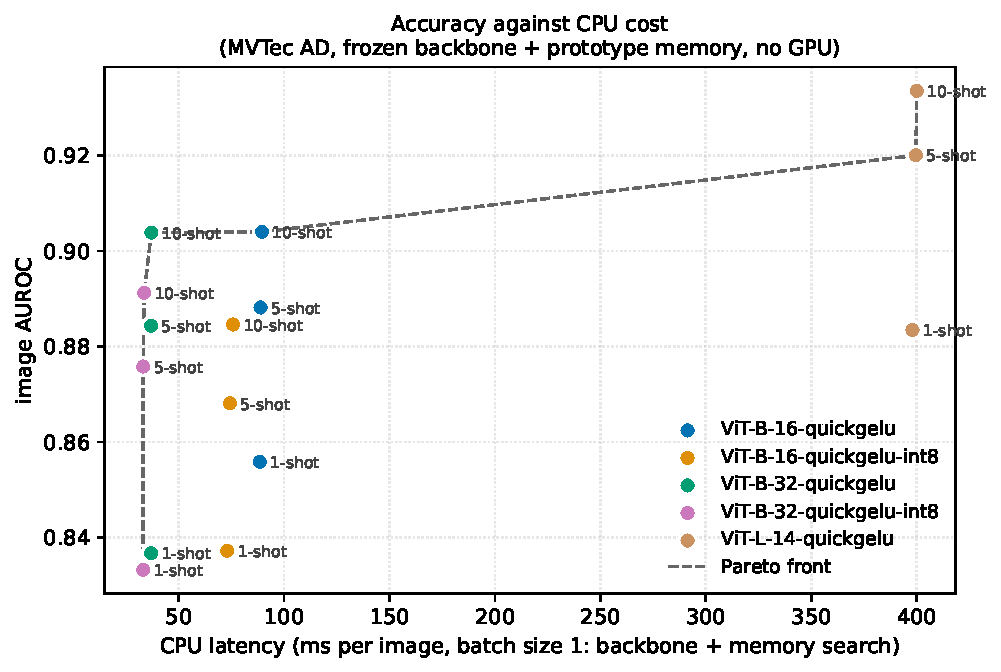
\includegraphics[width=\columnwidth]{figures/frontier_mvtec.pdf}
\caption{MVTec AD image AUROC against CPU time per image (encoder plus memory
search), PyTorch FP32 (filled) and ONNX INT8 (hollow); numbers are photos per
product. Multi-layer points are without windows. Dashed:
Pareto front. Record: \texttt{figures.json}.}
\label{fig:frontier}
\end{figure}

On a cool machine, one image takes 37\,ms with B/32 (3.0 GFLOPs), 88\,ms with B/16
(11.3) and 397\,ms with L/14 (52.0). Searching the memory adds 0.3--2.9\,ms, about
1\%, so using ten photos instead of one is effectively free
(Fig.~\ref{fig:frontier}). The multi-layer B/16 takes 94--97\,ms in two runs
(\texttt{ml\_latency.json}): the earlier blocks are computed in any case and are
only kept, and the search over three-times-longer vectors takes 4.4--5.0\,ms with
ten photos. Its five- and ten-photo points lie on the Pareto front, more
accurate than L/14 at a quarter of its time. The inspector needs 1.5\,GB of RAM in PyTorch with B/32
or B/16, 3.7\,GB with L/14, and 0.38\,GB for the INT8 ONNX encoder. Under continuous
use the picture changes. B/32 held 40\,ms for four minutes; then the CPU clock
dropped and it settled at about 230\,ms, 5.8 times slower. B/16 and L/14, measured
on the already warm machine, ran at 630--680\,ms and about 2\,s. Capacity should
be planned on these figures. Even so, at 10,000 parts a day the laptop is busy
for at most 1.8 hours with B/16 (5.6 with L/14). At 45\,W and Rs~8 per kWh this
costs Rs~9.80 a year with B/32 INT8 and Rs~26 with B/16; the hardware already
exists. All benchmarks in this study used at least 6.8 CPU-hours and no GPU.

\subsection{Verification}
Re-extracting every feature from the raw images reproduced all 135 MVTec AD
(B/16) and 108 VisA (B/32) result rows to within 0.0002. On the second author's
laptop, a fresh install from the pinned requirements passed all tests and
reproduced the MVTec AD and VisA tables to three decimals; NEU-DET, produced on
that laptop, was reproduced on the first author's machine to within 0.0005, and
its split files regenerated byte-identically. The Colab notebook reproduces one
product's results exactly. For the multi-layer encoder, a unit test checks that
asking for block 12 alone returns the original features, and block 12 sliced out
of the cached multi-layer MVTec AD features matched the original features with
cosine similarity 1.0.

\section{Discussion}

\paragraph{What a workshop should do.} Photograph ten good parts rather than one:
the extra photos cost nothing at inference and halve the run-to-run spread. Use
B/32, or its INT8 version, if the defects that matter are larger than about 2\%
of the photo; otherwise use B/16 with multi-layer features and windows, checking
on a few known defects that the multi-layer features help on that product, since
on NEU-DET and MPDD they did not. Add a defect description only when
the product has a clear notion of normal. Expect a laptop to run several times
slower than its first-minute speed once it has warmed up.

\paragraph{Threats to validity.} The benchmarks are photographed under controlled
light, so they say little about a shop floor; MPDD is closer, but still a
curated set. Our main tables use three seeds, fewer than WinCLIP's five; only the
WinCLIP comparison uses five. We fixed the blocks in advance, but we decided to try
multi-layer features after seeing PatchCore's lead in localisation, and they
helped on two of the four datasets. The NEU-DET protocol is our own. All timings come from one laptop
model; a different cooling design will throttle differently. The suggested
threshold is a heuristic: in the application it rejected 9 of 20 good bottles with
five photos, and with three photos of \texttt{metal\_nut} it missed every defect.

\section{Limitations and future work}
Defects thinner than a patch remain hard (\texttt{screw} reaches 0.792 with L/14).
We compared with WinCLIP+'s published numbers rather than re-running it, did
not run AnomalyCLIP, did not export the multi-layer encoder to INT8 or test static
INT8, and did not collect photographs from a real workshop; the last is the most
important next step. A
calibrated threshold, for example one that fixes the expected false-reject rate,
would make the application safer to use unattended.

\section{Conclusion}
A frozen CLIP encoder and a per-product memory of good patches can inspect parts
from ten photographs on an ordinary laptop. With patch tokens from three of the
encoder's blocks, its detection is better than PatchCore's given the same photos
on all three datasets where we ran PatchCore, its localisation is level on MVTec
AD, and a new product can be added in seconds without changing anything about the
others. The cost results matter as much as the
accuracies: choose the backbone by defect size, and plan on the throttled speed.

\section*{Use of AI tools}
An AI assistant (Claude, Anthropic) was used during this project to help write
code, run and organise experiments, and draft and edit text, including this paper.
All experiments were run on our hardware, every number was checked against the
result files in the repository, and the authors take responsibility for the
content.

\paragraph{Reproducibility.} Code, split files, result records and one command per
table (\texttt{python scripts/reproduce.py --list}):
\url{https://github.com/Mounika-Reddy-0802/fewshot-msme-inspect}.

\bibliographystyle{plain}
\bibliography{refs}
\end{document}
